\documentclass[preprint,12pt,a4paper]{elsarticle}

\newcommand{\method}{\textsc{Ypath\-RAG}}

\usepackage{amssymb}
\usepackage{amsmath}
\usepackage[ruled,vlined]{algorithm2e}
\DontPrintSemicolon

\usepackage{booktabs}
\usepackage{float}
\usepackage{graphicx}
\usepackage{url}
\usepackage[section]{placeins}
\usepackage{tabularx}
\usepackage{siunitx}
\sisetup{
  detect-weight=true,
  detect-inline-weight=math,
  detect-family=true
}

\usepackage{enumitem}
\usepackage{pifont}
\newcommand{\cmark}{\ding{51}}
\newcommand{\xmark}{\ding{55}}

\journal{Biomedical Signal Processing and Control}
\biboptions{numbers,sort&compress}

\begin{document}
\begin{frontmatter}

\title{YpathRAG: Supportiveness-Aware Evidence Retrieval and Reranking for Pathology Question Answering}

\author[inst1]{Deshui Yu\fnref{fn_equal}}

\author[inst1]{Yizhi Wang\fnref{fn_equal}}

\author[inst2]{Saihui Jin\fnref{fn_equal}}

\author[inst1]{Taojie Zhu}

\author[inst1]{Fanyi Zeng}

\author[inst1]{Wenxiao Ma}

\author[inst1]{Wen Qian}

\author[inst1]{Zirui Huang}

\author[inst1]{Jingli Ouyang}

\author[inst1]{Jiameng Li}

\author[inst3]{Zhen Song}

\author[inst1]{Tian Guan}

\author[inst1]{Yonghong He\corref{cor1}}
\ead{heyh@sz.tsinghua.edu.cn}

\affiliation[inst1]{organization={Tsinghua Shenzhen International Graduate School, Tsinghua University},
            addressline={University Town},
            city={Shenzhen 518055},
            country={China}}

\affiliation[inst2]{organization={China Unicom Guangdong Branch},
            city={Guangzhou},
            state={Guangdong},
            country={China}}

\affiliation[inst3]{organization={Department of Network Intelligence, Peng Cheng Laboratory},
            city={Shenzhen 518055},
            country={China}}

\fntext[fn_equal]{These authors contributed equally to this work.}
\cortext[cor1]{Corresponding author.}

\begin{abstract}
Evidence retrieval for pathology question answering suffers from a fundamental objective mismatch: relevance-oriented ranking often conflates aboutness with supportiveness, causing passages that appear related yet cannot justify an answer to outrank truly evidential ones. We propose \textsc{YpathRAG}, a supportiveness-first retrieval and reranking framework. In the first stage, \textsc{YpathRAG} uses dense retrieval as the primary channel and augments it with a lexicon-guided sparse retriever to improve robustness to terminological variation and evidence reachability. In the second stage, \textsc{YpathRAG} introduces a \emph{Supportive Evidence Verifier} (SEV) that reranks a fixed candidate pool without increasing retrieval depth by fusing retrieval scores with dual-head predictions to jointly model whether a passage is supportive and how strongly it supports the query. We evaluate \textsc{YpathRAG} along three complementary axes: corpus-level retrieval on a 1.53M-passage pathology corpus, a dedicated reranking benchmark with targeted confusable negatives, and a downstream QA benchmark. On \textsc{YpathR}, \textsc{YpathRAG} achieves 0.9864 Precision@5, and on corpus-level retrieval it improves nDCG@10 from 0.3368 to 0.3972 over hybrid retrieval. Across settings, \textsc{YpathRAG} improves the supportiveness and coverage of top-ranked evidence without increasing retrieval depth.
\end{abstract}

\begin{keyword}
supportiveness-aware retrieval \sep evidence reranking \sep hybrid retrieval \sep pathology question answering \sep retrieval-augmented generation
\end{keyword}

\end{frontmatter}

\section{Introduction}
Evidence retrieval for pathology question answering suffers from a fundamental objective mismatch: relevance-oriented ranking often conflates \emph{aboutness} with \emph{supportiveness}, causing passages that appear related yet cannot justify an answer to outrank truly evidential ones. This mismatch is particularly consequential in high-stakes medical settings, where downstream generation is only as reliable as the evidence it is grounded in. Pathology QA exemplifies the challenge: evidence is terminology-heavy, context-dependent, and frequently expressed through long-tail variants, abbreviations, and mixed-language phrasing. Consequently, conventional retrieval pipelines often return passages that look relevant but provide limited actionable support for clinical reasoning or guideline-level conclusions. This underscores the need for a new approach to pathology QA that can combine high-coverage evidence retrieval with verifiable evidence grounding.

Two obstacles are particularly acute for pathology evidence retrieval. 
First, terminological barriers make lexical matching and tokenization brittle. 
Domain terms exhibit non-standard surface forms, inconsistent segmentation, and rare variants; when queries and passages diverge in expression, both sparse lexical matching and dense semantic retrieval can degrade~\cite{robertson2009bm25,karpukhin2020dpr,xiong2021ance,dai2020deepct,khattab2020colbert}. 
Second, and more fundamentally, relevance is not supportiveness. 
Relevance-oriented objectives prioritize topical similarity, but evidence retrieval for medical QA requires passages that can \emph{justify} an answer. 
As illustrated in Fig.~\ref{fig:motivation}, optimizing aboutness (relevance) does not guarantee supportiveness: top-ranked results can be \emph{about} the query while remaining non-supportive---for example, providing only background without explicit diagnostic criteria, addressing a different disease stage, or citing outdated or region-mismatched recommendations. 
Such ``relevant-but-non-supportive'' cases systematically occupy early ranks and dilute the evidence that downstream generation can safely rely on~\cite{gao2023ragsurvey,thorne2018fever}.

\begin{figure}[t]
  \centering
  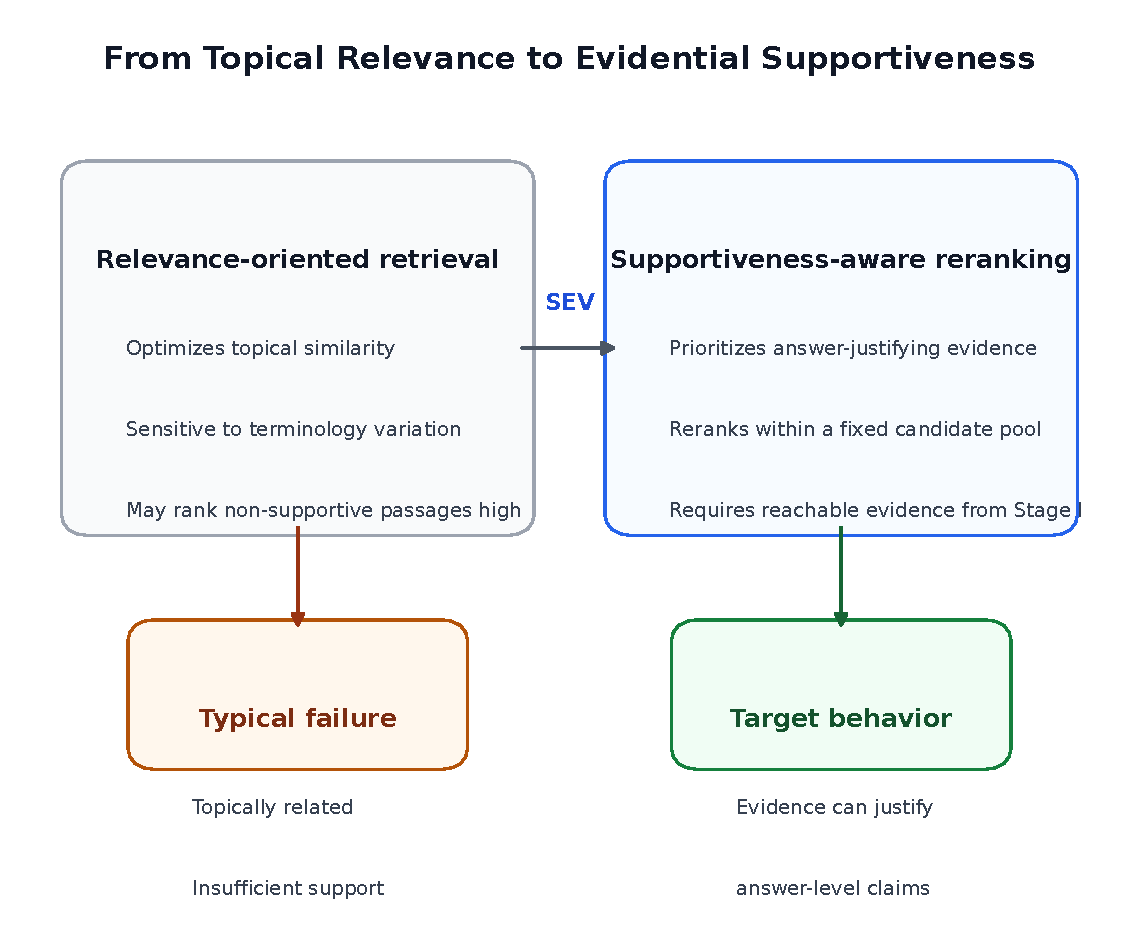
\includegraphics[width=\columnwidth]{figure/motivation.pdf}
  \caption{Motivation via contrast. Left: conventional relevance-oriented retrieval optimizes topical similarity and may surface non-supportive passages under terminology variation. Right: supportiveness-aware reranking and verification aim to prioritize answer-justifying evidence within a fixed candidate pool.}
  \label{fig:motivation}
\end{figure}

We propose \textsc{YpathRAG}, a supportiveness-first retrieval and reranking framework for pathology QA. 
In the first stage, \textsc{YpathRAG} uses dense retrieval as the primary channel and augments it with a lexicon-guided sparse retriever to improve robustness to terminological variation and evidence coverage. 
Concretely, we curate a pathology domain lexicon and use it to guide terminology-aware segmentation and lexicon-driven matching/expansion in the sparse channel, improving recall under long-tail variants and mixed-language phrasing. 
The dense encoder is kept unchanged and operates on the original text, while the hybrid stage produces a candidate pool that is both semantically relevant and lexically robust. 
\begin{figure*}[t]
  \centering
  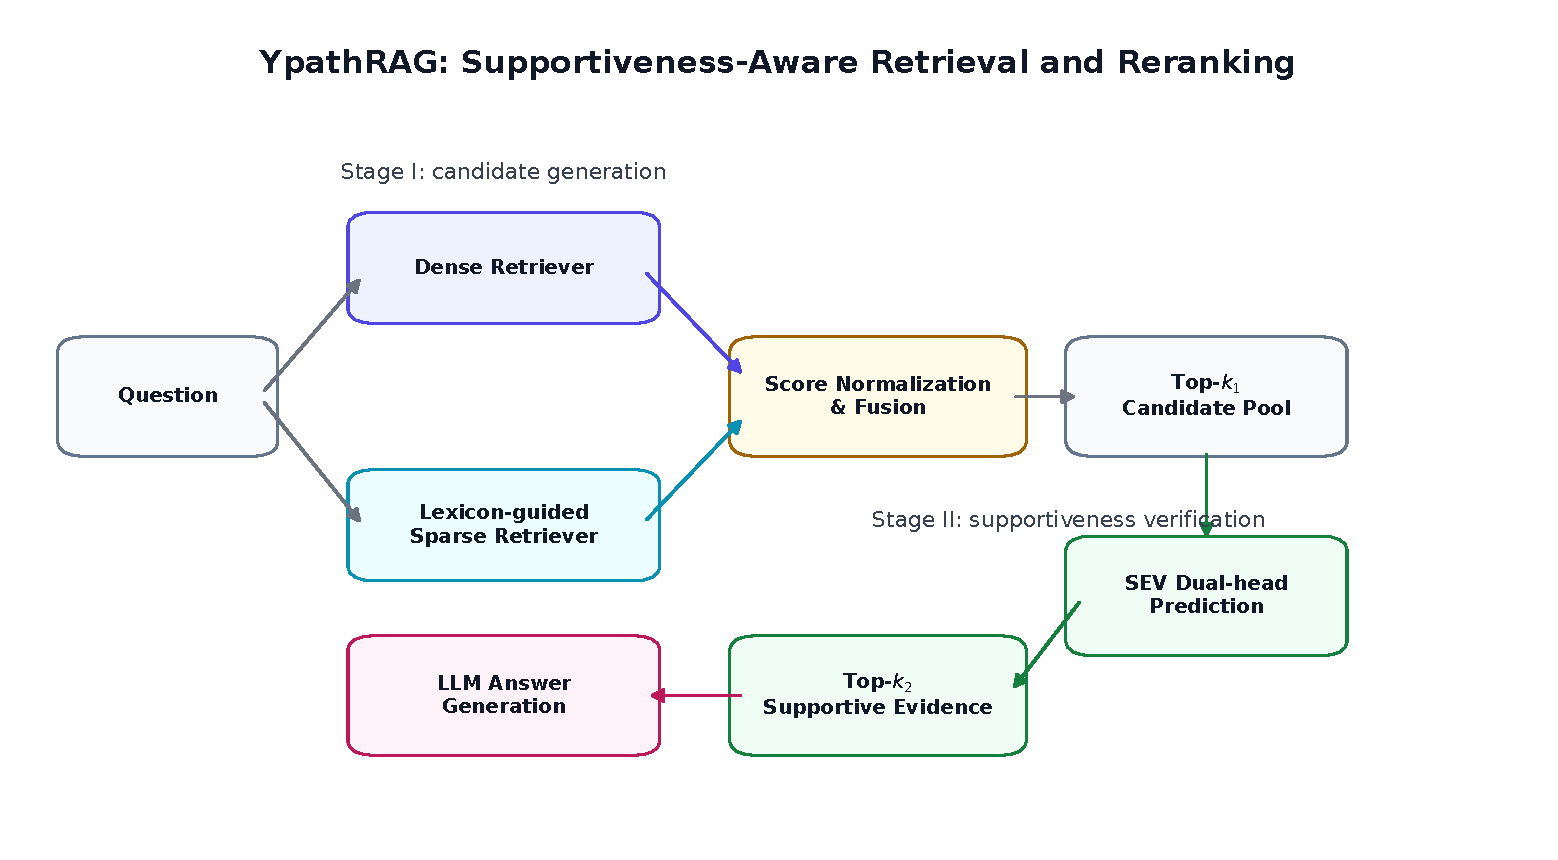
\includegraphics[width=\textwidth]{figure/framework.pdf}
  \caption{Overview of \textsc{YpathRAG}. A dual-channel hybrid retriever (dense + lexicon-guided sparse) retrieves a fixed top-$k_1$ candidate pool, followed by a Supportive Evidence Verifier (SEV) that reranks within the pool using dual-head predictions (supportive vs.\ non-supportive and graded support strength), producing top-$k_2$ supportive evidence for downstream QA without increasing retrieval depth.}
  \label{fig:framework}
\end{figure*}
In the second stage, \textsc{YpathRAG} introduces a \emph{Supportive Evidence Verifier (SEV)} that reranks a fixed candidate pool---without increasing retrieval depth---by fusing retrieval scores with dual-head predictions to jointly model (i) whether a passage is supportive and (ii) the strength of its support for the query. 
Fig.~\ref{fig:framework} summarizes the overall pipeline and the two-stage design.



We evaluate \textsc{YpathRAG} along three complementary axes: (i) corpus-level retrieval on a 1.53M-passage pathology corpus under a single-anchor relevance protocol; (ii) a dedicated reranking benchmark with targeted confusable negatives to diagnose ``relevant-but-non-supportive'' failure modes; and (iii) a QA benchmark to quantify end-to-end gains on real LLMs when grounded in retrieved evidence.

We make four contributions:
\begin{itemize}
  \item We highlight and operationalize the objective mismatch between \emph{aboutness} and \emph{supportiveness} in pathology evidence retrieval, motivating supportiveness-first ranking for pathology QA.
  \item We construct a large-scale pathology evidence corpus comprising approximately 1.53M semantically coherent passages from 406 reference books and 7{,}508 journal/conference papers across 28 pathology subfields.
  \item We propose \textsc{YpathRAG}, a two-stage framework that combines dense retrieval with a \emph{curated lexicon-guided} sparse channel for robust candidate generation, and introduces SEV with dual-head predictions and score fusion to rerank a fixed candidate pool without increasing retrieval depth.
  \item We provide complementary evaluation protocols and benchmarks, including large-corpus retrieval under the \textsc{P1-Anchor Corpus Protocol}, confusable-negative reranking diagnosis, and downstream QA evaluation for external validity.
\end{itemize}



\section{Related Work}
\label{sec:related}

\subsection{LLMs for Medical and Pathology QA: Evidence Use Limitations}
Large language models (LLMs) have shown strong potential in medical question answering, clinical decision-making, and reasoning tasks~\cite{singhal2023llm4clinical,lievin2024canllmsreasonmedical}.
Pathology, however, remains particularly challenging: its texts are terminology-dense and structurally complex, and models may exhibit semantic drift or factual errors on fine-grained concepts such as subtyping, staging, and diagnostic criteria~\cite{luo2022biogpt,wu2023pmcllama}.
Moreover, pathology practice is shaped by evolving guidelines and context-specific criteria, making static domain adaptation insufficient in practice.
As a result, LLMs may produce fluent but weakly grounded answers on specialized pathology queries, highlighting the need to anchor responses in \emph{traceable and verifiable supporting evidence} that can be verified at the passage level.
This shifts the bottleneck from generation alone to an IR-centric problem: retrieving and ranking passages that can \emph{support} an answer.

\subsection{Retrieval-Augmented Generation and Retrieval Paradigms in Specialized Domains}
Retrieval-augmented generation (RAG) incorporates external retrieval into generation to improve factuality and controllability~\cite{lewis2020rag,izacard2021leveraging,gao2023ragsurvey}, and can also be viewed more broadly as retrieval-enhanced modeling in which generation is conditioned on retrieved context~\cite{guu2020realm}.
In specialized domains such as pathology, the bottleneck often arises in retrieval: candidate pools may contain many passages that are topically related yet fail to provide decisive evidence, which then propagates noise into downstream generation.
Pure dense semantic matching may miss critical terminology and conditional constraints when surface forms diverge, while sparse matching is sensitive to tokenization and term instability~\cite{robertson2009bm25}.

These observations motivate \emph{hybrid} retrieval that combines dense and sparse signals.
In IR practice, hybridization is commonly implemented either via \emph{score fusion} (e.g., linear interpolation of dense and lexical scores) or via \emph{rank fusion} such as Reciprocal Rank Fusion (RRF)~\cite{cormack2009rrf}.
Beyond classical sparse retrievers, recent \emph{learned sparse} models (e.g., SPLADE~\cite{formal2021splade} and DeepImpact~\cite{mallia2021deepimpact}) and contextualized lexical matching (e.g., COIL~\cite{gao2021coil}) offer stronger sparse channels while retaining inverted-index efficiency.
Hybrid dense--sparse retrieval has also been empirically shown to be complementary for QA-style retrieval, improving candidate recall/coverage compared to using either signal alone~\cite{karpukhin2020dpr}.
Our work builds on this line by tailoring the sparse channel with a curated pathology lexicon to stabilize matching under terminology variation, and by separating \emph{candidate coverage} from \emph{supportiveness} in the subsequent reranking stage.
Medical and clinical RAG systems have explored external knowledge grounding for biomedical QA and diagnostic reasoning, but pathology-oriented textual RAG remains underdeveloped.
Existing resources are often image-centric or task-specific, while large-scale text-centric corpora, retrieval benchmarks, and supportiveness-aware evidence verification remain limited.
This motivates our focus on pathology evidence retrieval rather than post-hoc generation correction.


\subsection{From Relevance to Supportiveness: Evidence Selection and Reranking}
A growing body of work treats evidence-grounded QA as an evidence selection problem, where the key is not only retrieving passages \emph{about} the query but ranking those that can \emph{justify} an answer~\cite{gao2023ragsurvey,thorne2018fever}.
This distinction is especially salient in medical QA: many high-ranked passages are topically related yet non-supportive (e.g., background-only descriptions or criteria-mismatched guidance), which can crowd out answer-justifying evidence at the top ranks.


From an IR perspective, addressing this mismatch typically calls for (i) candidate generation that is robust to terminology variation, and (ii) reranking/verification mechanisms that explicitly model \emph{supportiveness}.

While dense retrievers and hybrid retrieval improve reachability, they do not by themselves resolve the objective mismatch at the top ranks.
Therefore, supportiveness-aware reranking can be viewed as a complementary second-stage component that promotes answer-justifying passages within a \emph{fixed} candidate pool, rather than relying on deeper retrieval.
Our work follows this direction by combining pathology-oriented hybrid retrieval with a supportiveness-aware verifier (SEV) and by providing reproducible large-scale retrieval evaluation and a confusable-negative reranking benchmark tailored to ``relevant-but-non-supportive'' failure modes.

\section{Method}
\label{sec:method}

\subsection{Problem Formulation}
\label{sec:method:formulation}
We study evidence retrieval for pathology question answering under a \emph{supportiveness-first} objective.
Given a pathology question $q$ and a large corpus $\mathcal{D}$ (1.53M passages), the goal is to return a small set of evidence passages that can \emph{substantiate} the answer rather than merely being topically related.
This differs from conventional IR settings where topical relevance is the dominant target: in pathology QA, many high-ranked passages are ``about'' the disease yet fail to provide actionable criteria, correct spatiotemporal constraints, or complete support.

We decompose evidence selection into two stages:
(1) candidate generation retrieves a top-$k_1$ candidate set $C_{k_1}(q)\subset \mathcal{D}$ with high recall under severe terminology variation;
(2) supportiveness-aware reranking reorders $C_{k_1}(q)$ to obtain a top-$k_2$ evidence set $E_{k_2}(q)$ that prioritizes truly supportive evidence for downstream QA.

\subsection{Stage I: Dual-Channel Candidate Generation}
\label{sec:method:cand}
To handle terminology density and long-tail variants in pathology text, we adopt a dual-channel retrieval scheme that combines a dense semantic retriever with a lexicon-guided sparse retriever.

\paragraph{Dense retriever}
We encode the query and each passage using a dense encoder and compute cosine similarity
$s_{\text{dense}}(q,p)$.
The dense channel provides robust semantic matching but can miss crucial pathology-specific expressions (abbreviations, mixed-language terms, rare variants), leading to false negatives.

\paragraph{Lexicon construction and sparse expansion}
To broaden recall coverage of domain entities and long-tail terminology, we construct a pathology-specific lexicon and use it to drive the sparse channel.
Concretely, we start from the open-source \emph{chinese\_medical\_words} list~\cite{xtea_chinese_medical_words} as a seed vocabulary, tokenize the 1.53M-passage corpus, and retain seed entries with corpus frequency greater than 30 (about $36{,}000$ terms). We use a frequency threshold of 30 as a conservative heuristic to exclude rare noise tokens.
We then mine out-of-vocabulary candidates that also appear more than 30 times but are absent from the seed list, and filter them with GPT\textnormal{-}4o under a fixed rubric to keep only semantically complete and domain-meaningful terms (about $24{,}000$).
Merging both sets yields a $\sim\!60{,}000$-term pathology lexicon $\mathcal{V}_{\text{path}}$.
The sparse channel runs BM25 with lexicon-guided tokenization and lexicon expansion, so that terminology-anchored passages (e.g., rare subtypes, markers, or staging phrases) remain retrievable even when dense retrieval misses them.
The goal of this channel is to reduce terminology-induced false negatives and improve candidate coverage; fine-grained ranking is handled by SEV in Stage~II.


\paragraph{Score normalization and hybrid fusion}
Because dense and sparse scores are not directly comparable, we apply query-wise min--max normalization within each channel's retrieved list before fusion.
\begin{equation}
\label{eq:norm}
\widehat{s}(q,p)=\mathrm{Norm}\big(s(q,p)\big)\in[0,1].
\end{equation}
We then compute a hybrid retrieval score:
\begin{equation}
\label{eq:hybrid}
s_{\text{retr}}(q,p)=w_d\cdot \widehat{s}_{\text{dense}}(q,p)+w_s\cdot \widehat{s}_{\text{sparse}}(q,p),
\quad w_d+w_s=1,
\end{equation}
and select the top-$k_1$ passages by $s_{\text{retr}}$ to form $C_{k_1}(q)$.
In our main setting, we use $k_1{=}1000$ and a dense-dominant fusion ($w_d{=}0.8,\,w_s{=}0.2$) to preserve semantic precision while benefiting from lexicon-guided recall.

\subsection{Stage II: Supportive Evidence Verifier (SEV)}
\label{sec:method:sev}
Candidate generation improves reachability, but it does not resolve the core mismatch between topical relevance and evidential support.
We therefore introduce a \textbf{Supportive Evidence Verifier (SEV)} to explicitly model supportiveness for each candidate passage.

\paragraph{Dual-head modeling of supportiveness}
For each query--passage pair $(q,p)$, SEV outputs two complementary signals:
\begin{itemize}
  \item \textbf{Supportiveness classification} $p_{\text{cls}}(q,p)\in[0,1]$:
  the probability that $p$ can serve as supporting evidence for answering $q$.
  \item \textbf{Support strength score} $p_{\text{score}}(q,p)\in[0,1]$:
  a scalar score indicating how strongly $p$ supports answering $q$.
\end{itemize}
Intuitively, $p_{\text{cls}}$ answers ``\emph{does it support?}'', while $p_{\text{score}}$ refines ``\emph{how strongly does it support?}''.
This separation is crucial in pathology retrieval where many passages are superficially related yet non-supportive (e.g., background-only, vague criteria, outdated versions/regions, or adjacent stages).

\paragraph{Training supervision}
We derive supportiveness supervision from our benchmark construction:
passages are labeled as supportive (\textsc{P1--P3}) or non-supportive (\textsc{A1--A4}), and each passage is assigned a supportiveness score $y_{\text{score}}$ (obtained via GPT-based grading under a fixed rubric).
All GPT-based filtering/grading uses a fixed rubric and deterministic decoding, and the rubric, prompts, and sampled audits will be made available upon publication to support reproducibility.
SEV is trained on $(q,p)$ pairs with a multi-task objective:
\begin{equation}
\label{eq:sev_loss}
\mathcal{L}_{\text{SEV}}
=
\lambda_{\text{cls}}\cdot \mathcal{L}_{\text{BCE}}\big(p_{\text{cls}}(q,p),\,y_{\text{cls}}\big)
+ \lambda_{\text{score}}\cdot \mathcal{L}_{\text{reg}}\big(p_{\text{score}}(q,p),\,y_{\text{score}}\big),
\end{equation}
where $y_{\text{cls}}\in\{0,1\}$ indicates whether the passage is supportive and $\mathcal{L}_{\text{reg}}$ is a regression loss on the support-strength output.
Unless otherwise stated, we set $\lambda_{\text{cls}}=\lambda_{\text{score}}=1.0$.
Here $\lambda_{\text{cls}}$ and $\lambda_{\text{score}}$ weight the \emph{training losses}, while $w_{\text{retr}}, w_{\text{score}}, w_{\text{cls}}$ weight the \emph{inference-time fusion} in Eq.~\eqref{eq:fusion_final}.

We implement SEV with an instruction-tuned LLM backbone (\mbox{Qwen2.5-Instruct-7B}) and parameter-efficient fine-tuning (LoRA) so that the verifier can learn pathology-specific evidence discrimination while remaining deployable.

\paragraph{SEV training protocol}
For SEV, we fine-tune \emph{\mbox{Qwen2.5-Instruct-7B}} with \emph{LoRA} on \emph{YpathR}.
We adopt a \emph{90\%/10\%} split of \emph{YpathR}, using ninety percent for training and holding out the remaining ten percent strictly for testing; no test questions or passages are seen during training.
All splits are performed by queries (not by individual query--passage pairs) to avoid leakage.
Unless otherwise stated, training hyperparameters are \texttt{max\_length}$=512$, \texttt{batch\_size}$=1$, learning rate $=10^{-5}$, and \texttt{num\_epochs}$=3$.
Selection-related hyperparameters (e.g., the support threshold $\tau$) are tuned on a development subset carved out from the 90\% training split, with the 10\% test split held out throughout.
We use LoRA with rank $r{=}16$, scaling $\alpha{=}32$, dropout $=0.05$, and apply adapters to \texttt{q\_proj, k\_proj, v\_proj, o\_proj}.

\subsection{Supportiveness-Aware Fusion Reranking}
\label{sec:method:fusion}
Given the candidate set $C_{k_1}(q)$, we compute a final reranking score by fusing the (normalized) retrieval score with SEV's dual-head outputs.
Concretely, for each $p \in C_{k_1}(q)$, we apply min--max normalization to retrieval scores within the same query:
\begin{equation}
\label{eq:retr_norm}
\begin{aligned}
\mathrm{norm}\big(s_{\text{retr}}(q,p)\big)
&=
\frac{s_{\text{retr}}(q,p)-m_q}
{M_q-m_q+\epsilon}, \\
m_q &= \min_{p'\in C_{k_1}(q)} s_{\text{retr}}(q,p'), \\
M_q &= \max_{p'\in C_{k_1}(q)} s_{\text{retr}}(q,p').
\end{aligned}
\end{equation}
where $\epsilon$ is a small constant for numerical stability.
SEV outputs two signals: a support-strength score $p_{\text{score}}(q,p)$ (implemented as \texttt{score\_prob}) and a supportive/non-supportive probability $p_{\text{cls}}(q,p)$ (implemented as \texttt{cls\_prob}).
We then compute:
\begin{equation}
\label{eq:fusion_final}
\begin{aligned}
s_{\text{final}}(q,p)
&=
w_{\text{retr}}\cdot \mathrm{norm}\big(s_{\text{retr}}(q,p)\big) \\
&\quad + w_{\text{score}}\cdot p_{\text{score}}(q,p)
      + w_{\text{cls}}\cdot p_{\text{cls}}(q,p).
\end{aligned}
\end{equation}
Unless otherwise stated, we use $w_{\text{retr}}{=}1.0$, $w_{\text{score}}{=}2.0$, and $w_{\text{cls}}{=}0.45$ (selected via ablation on a held-out development split), and return the top-$k_2$ passages ranked by $s_{\text{final}}(q,p)$ (with $k_2{=}3$ in our main setting).
In practice, a query may be supported by multiple passages in the corpus; our corpus-level evaluation therefore adopts a conservative single-anchor protocol for reproducibility, while a controlled benchmark (\textsc{YpathR}) diagnoses fine-grained supportiveness discrimination under confusable negatives.

\begin{algorithm}[H]
\caption{\textsc{YpathRAG}: Retrieval and Supportiveness-Aware Reranking}
\label{alg:ypathrag}
\KwIn{query $q$; corpus $\mathcal{D}$; lexicon $\mathcal{V}_{\text{path}}$; dense encoder $f_{\text{dense}}$; sparse retriever $\textsc{BM25}_{\mathcal{V}_{\text{path}}}$; weights $(w_d,w_s)$; $k_1$; SEV $\textsc{SEV}_\theta$; fusion weights $(w_{\text{retr}}, w_{\text{score}}, w_{\text{cls}})$; $k_2$.}
\KwOut{evidence set $E_{k_2}(q)$.}

\textbf{Stage I: Candidate generation}\;
Retrieve dense candidates and scores $s_{\text{dense}}(q,p)$\;
Retrieve sparse candidates and scores $s_{\text{sparse}}(q,p)$ with $\textsc{BM25}_{\mathcal{V}_{\text{path}}}$\;
$\widehat{s}_{\text{dense}}\leftarrow \mathrm{Norm}(s_{\text{dense}})$;\;
$\widehat{s}_{\text{sparse}}\leftarrow \mathrm{Norm}(s_{\text{sparse}})$\;
$s_{\text{retr}}(q,p)\leftarrow w_d\widehat{s}_{\text{dense}}(q,p)+w_s\widehat{s}_{\text{sparse}}(q,p)$\;
$C_{k_1}(q)\leftarrow \mathrm{TopK}(s_{\text{retr}}, k_1)$\;

\textbf{Stage II: SEV inference}\;
\For{$p \in C_{k_1}(q)$}{
  $(p_{\text{cls}}(q,p),p_{\text{score}}(q,p)) \leftarrow \textsc{SEV}_\theta(q,p)$\;
}

\textbf{Fusion reranking}\;
Compute $\mathrm{norm}(s_{\text{retr}}(q,p))$ by Eq.~\eqref{eq:retr_norm}\;
\For{$p \in C_{k_1}(q)$}{
  $s_{\text{final}}(q,p)\leftarrow
  w_{\text{retr}}\cdot \mathrm{norm}(s_{\text{retr}}(q,p))
  + w_{\text{score}}\cdot p_{\text{score}}(q,p)
  + w_{\text{cls}}\cdot p_{\text{cls}}(q,p)$\;
}
$E_{k_2}(q)\leftarrow \mathrm{TopK}(s_{\text{final}}, k_2)$\;
\end{algorithm}

\subsection{Evidence Packaging for Downstream QA}
\label{sec:method:qa_optional}
Although our primary contribution is supportiveness-aware evidence retrieval and reranking, the resulting evidence set $E_{k_2}(q)$ can be directly fed into an evidence-conditioned generator.
In all downstream experiments, generation is performed with a fixed prompting protocol and a fixed evidence budget $k_2$ to isolate the effect of evidence quality.

\section{Corpus and Benchmarks}
\label{sec:corpus_bench}

\subsection{Data Sources and Ingestion}
\label{subsec:ingestion}
Our corpus is built from scholarly publications obtained through institutional access and public academic platforms, covering three complementary streams:
(i) SCI-indexed journal articles (primarily within the past ten years to reflect recent practice);
(ii) flagship pathology journals and conference proceedings (extended up to the past twenty years to include consensus statements and milestone works);
and (iii) curated pathology reference books (monographs, textbooks, and guideline compendia).
In total, we collect 406 reference books and 7{,}508 journal/conference papers spanning 28 pathology subfields.
Candidate sources are retrieved using pathology-specific controlled keywords on major indices and publisher platforms, followed by standardized de-duplication, normalization, and consistency checks before ingestion.
All documents are used under institutional subscriptions or public access, and we index only extracted text for retrieval research.
We canonicalize metadata (title/venue/year/DOI when available) and de-duplicate at both document and passage levels (Sec.~\ref{subsec:corpus_construction}).
To respect licensing constraints, we do not redistribute copyrighted full texts; we release only derived artifacts needed for research reproducibility (e.g., identifiers, metadata, qrels, run files, and code).

\subsection{Corpus Construction and Indexing Units}
\label{subsec:corpus_construction}
We construct a text-centric pathology corpus via a unified pipeline that converts raw PDFs into \emph{semantically coherent, retrievable passages}.
The key design goal is to make each indexed unit self-contained and evidence-ready, rather than merely length-bounded.

\paragraph{OCR and structured extraction}
We perform OCR and structured text extraction for both scanned and born-digital PDFs, explicitly handling multi-column layouts, figure/table captions, footnotes, and mixed fonts while recovering paragraph boundaries~\cite{smith2007tesseract,lopez2009grobid}.
Our pipeline is tool-agnostic in principle; in our implementation, the key requirement is recovering paragraph-level structure consistently across layouts.

\paragraph{LLM-driven semantic chunking (indexing units)}
Instead of fixed-length or embedding-driven splitting, we invoke an LLM to segment text into \emph{minimal retrievable units} under two constraints:
(\textit{i}) each passage focuses on a single topic, and (\textit{ii}) the semantics are complete on their own.
Contiguous content fragmented by pagination or line breaks is merged to restore semantic continuity.
This yields indexing units that better preserve medical definitions, criteria, and conditional statements.
We use a fixed prompting rubric and deterministic decoding, together with deterministic post-processing, to ensure consistent chunk boundaries across documents.
Chunking is performed on corpus text only and does not use any benchmark questions, answers, or labels.

\paragraph{Normalization for self-contained evidence}
We further apply LLM-based polishing to remove noisy boilerplate (headers, footers, watermarks, page numbers) and to rewrite dropped subjects/pronouns into explicit referents, ensuring each passage remains interpretable out of context.
Polishing is restricted to formatting cleanup and coreference clarification; it is not allowed to introduce new medical facts.
We additionally generate a concise summary for auditing and display, while all retrieval experiments operate on the original passage text.

\paragraph{Deterministic identifiers, auditing, and de-duplication}
Each cleaned passage is assigned a deterministic identifier \texttt{text\_hash} by hashing normalized text (SHA1),
which serves as a stable external key for reproducibility and corpus-level auditing.
We run near-duplicate detection and cross-document fingerprinting~\cite{broder1997minhash,charikar2002simhash,indyk1998lsh},
and enforce hash-based de-duplication during insertion to avoid repeated content.
In the index, each passage is stored together with metadata (e.g., source file), the original text, and its summary.
We version the corpus snapshot and release the mapping from \texttt{text\_hash} to source metadata for reproducibility.

\paragraph{Dual representations for hybrid retrieval}
For every passage, we build two complementary retrieval channels: (i) dense embeddings for semantic matching, and (ii) a lexicon-aware sparse channel (BM25) for terminology-precise matching, enabling hybrid retrieval~\cite{robertson2009bm25,chen2024m3embedding}.
After consistency checks, the resulting corpus contains approximately 1.53M semantically coherent passages, forming the backbone for corpus-level retrieval evaluation and reranking.
The sparse channel is implemented as lexicon-aware BM25 driven by $\mathcal{V}_{\text{path}}$ (Sec.~\ref{sec:method:cand}).

\subsection{Pathology Lexicon Resource}
\label{subsec:lexicon_sparse}
We construct a pathology-specific lexicon $\mathcal{V}_{\text{path}}$ (about 60K terms) as part of our artifact to support lexicon-aware sparse retrieval.
Construction details and its use in BM25 tokenization/expansion are described in Sec.~\ref{sec:method:cand}.
The lexicon and derived reproducibility artifacts will be made available upon publication, subject to licensing constraints.

\subsection{Construction of Evaluation Benchmarks}
\label{subsec:benchmarks_construct}
To evaluate pathology-specific retrieval and quantify gains for evidence-grounded QA, we derive two benchmarks from the corpus with complementary purposes:
(i) \emph{corpus-level retrieval} on the full 1.53M-passage index to evaluate first-stage retrieval at realistic scale, and
(ii) a \emph{controlled reranking benchmark} (\textsc{YpathR}) with confusable negatives to diagnose ``relevant-but-non-supportive'' failures under a fixed candidate pool.

\subsubsection{Question construction}
We use GPT-4o as a grounded authoring assistant with access to provided source excerpts from real pathology documents~\cite{openai2024gpt4o} to draft high-difficulty, domain-specialized questions.
For each question, we extract a gold supporting span from the same source document, yielding question--answer--evidence triplets in the spirit of evidence-grounded QA datasets~\cite{thorne2018fever,lewis2020rag,izacard2021leveraging}.
To control variance and improve consistency, we follow a two-pass protocol: (i) generation with a fixed prompt and deterministic decoding, and (ii) an independent re-check in a fresh model session using a separate verification prompt that only sees the necessary excerpt-level evidence and the draft question.

\subsubsection{Passage construction (\textsc{YpathR})}
Given each question and its gold supporting span from the same source document, we construct a fixed candidate set by minimally rewriting or perturbing the gold passage to produce graded supportive variants (P1--P3) and targeted non-supportive hard negatives (A1--A4) under a fixed rubric.
Supportive candidates receive graded labels \textsc{P1--P3} by strength:
\textsc{P1} provides complete support covering all key points with direct textual evidence;
\textsc{P2} provides partial support covering only a subset of key points;
\textsc{P3} offers weak/background support that is topically related but not decisive.
Non-supportive candidates are structured hard negatives \textsc{A1--A4}:
\textsc{A1} topic mismatch but factually correct (other diseases/stages);
\textsc{A2} ambiguous statements lacking operational criteria;
\textsc{A3} spatiotemporal conflict (e.g., outdated versions/regions) or information-poor redundancy;
\textsc{A4} background-only descriptions such as prevalence without actionable evidence.
These confusable negatives are designed to be topically similar yet non-evidential, matching the failure modes we target in reranking~\cite{karpukhin2020dpr,xiong2021ance}.

\subsubsection{Support scoring and quality control}
All grading follows a fixed rubric and outputs a supportiveness score $y_{\text{score}}\in[0,1]$ together with a short rationale.
After passage generation, we start a fresh model session and re-present only the necessary inputs for independent grading.
GPT-4o then assigns each candidate: (i) a support label (\textsc{P1--P3} or \textsc{A1--A4}), (ii) $y_{\text{score}}$, and (iii) a brief rationale.
We adopt deterministic decoding and fixed prompts/rubrics throughout, and the rubrics, prompts, and sampled audits will be made available upon publication to support reproducibility.
To mitigate model-as-judge bias, we additionally perform sampled human audits on the constructed candidates and their labels/scores, confirming that the grading and construction criteria are broadly consistent with pathology evidence standards.

This produces the retrieval benchmark \textsc{YpathR}.
To assess downstream QA gains, we further estimate question difficulty with GPT-4o, select the 300 most challenging questions, and---conditioned on the original supporting spans---generate reference answers and keyword lists, forming the QA benchmark \textsc{YpathQA-M}~\cite{guu2020realm,wang2022selfinstruct}.
To reduce generator-specific bias, GPT-4o is used for benchmark construction and rubric-based grading, whereas downstream evaluation includes both GPT-4o and independently developed open-source general and medical LLMs.
All reference answers are span-grounded and used for consistent automatic evaluation, rather than as authoritative clinical advice.



\section{Experiments}
\label{sec:experiments}

We evaluate \method{} from three complementary perspectives.
First, we conduct corpus-level retrieval on a 1.53M-passage pathology corpus under a single-anchor relevance protocol, measuring whether the system can promote a canonical gold evidence passage in large-corpus search.
Second, we use a dedicated reranking benchmark (\textsc{YpathR}) with targeted confusable negatives to diagnose ``relevant-but-non-supportive'' failure modes and to train SEV.
Third, we evaluate end-to-end QA on \textsc{YpathQA-M} to quantify gains on real LLMs when answers are grounded in retrieved evidence.

\subsection{Corpus-level Retrieval on the 1.53M-passage Corpus}
\label{subsec:exp_corpus}

\subsubsection{Experimental Setup}
\label{subsubsec:exp_setup}
We evaluate \method{} under a corpus-level retrieval setting on a 1.53M-passage pathology corpus.
Our primary goal is to test whether supportiveness-aware reranking can improve evidence ordering in a realistic large-corpus scenario where exhaustive relevance annotation is infeasible.

The index contains $\sim$1.53M semantically coherent passages from pathology literature, each assigned a persistent \texttt{docid}.
We build both dense and lexicon-aware sparse representations to support dense, sparse, and hybrid retrieval.

Because many queries can be supported by multiple passages in the corpus, we adopt a conservative single-anchor evaluation for reproducibility (the \textsc{P1-Anchor Corpus Protocol}).
For each query, we align its P1 seed evidence to a unique corpus passage and mark this passage as the sole relevant \texttt{docid} (relevance $=1$), treating all other passages as non-relevant.
This yields 2{,}349 queries with exactly one anchor each.
As a result, the reported nDCG/MRR/Recall quantify the ability to promote a canonical P1 evidence anchor in corpus-level search; retrieving other supportive passages is counted as non-relevant, which may underestimate absolute effectiveness but enables deterministic, large-scale comparison.

In addition to corpus-level evaluation, we use \textsc{YpathR} as a controlled benchmark where each query is paired with a small set of supportive candidates (P1--P3) and confusable hard negatives (A1--A4) that mimic common retrieval failure modes.
This benchmark is used to train SEV and to diagnose whether reranking signals correctly address relevance--supportiveness confusion under targeted distractors.

All methods output standard TREC run files over the same query set.
We compute nDCG@10, MRR@10, and Recall@K using a TREC-style evaluator (\texttt{eval\_runs.py}) given fixed qrels and run files.

\subsubsection{Evaluation Metrics}
\label{subsubsec:exp_metrics}
We report standard corpus-level IR metrics: nDCG@10, MRR@10, and Recall@K for $K\in\{10,50,100\}$.
Under the \textsc{P1-Anchor Corpus Protocol}, each query has exactly one relevant passage.
Therefore, Recall@K reduces to an indicator of whether the unique P1 anchor appears in the top-$K$ ranked results, while nDCG@10 and MRR@10 primarily reflect how early the anchor is ranked.
We also report Recall@1000 to reflect whether the unique P1 anchor is covered by the Top-1000 candidate pool (i.e., candidate reachability at reranking depth).

\subsubsection{Compared Methods}
\label{subsubsec:exp_methods}
We compare four retrieval pipelines under a unified Top-1000 setting.
Each method outputs a ranked list over the same 1.53M corpus; when reranking is applied, it is performed within the fixed Top-1000 candidate pool (i.e., without expanding the pool):

\begin{itemize}[leftmargin=*]
  \item Dense: first-stage dense retrieval using BGE-M3 embeddings with cosine similarity~\cite{chen2024m3embedding}.
  \item Sparse: first-stage lexicon-aware BM25 retrieval with lexicon-guided tokenization/expansion driven by $\mathcal{V}_{\text{path}}$.
  \item Hybrid: linear fusion of dense and sparse scores with $(w_d,w_s)=(0.80,0.20)$ to produce a single fused ranking.
  \item Hybrid + SEV: supportiveness-aware reranking on the same Top-1000 candidate pool returned by Hybrid.
  For each candidate, SEV produces dual-head outputs and we compute a fused reranking score (Eq.~\ref{eq:fusion_final}) to reorder the Top-1000 list without expanding the candidate pool.
\end{itemize}


\subsubsection{Main Results (Top-1000)}
\label{subsubsec:exp_main_results}
Table~\ref{tab:main_top1000} summarizes the corpus-level retrieval results under the \textsc{P1-Anchor Corpus Protocol}.

\begin{table}[t]
  \centering
  \caption{Corpus-level retrieval results under the \textsc{P1-Anchor Corpus Protocol} (2,349 queries) at depth Top-1000.}
  \label{tab:main_top1000}
  \small
  \setlength{\tabcolsep}{3.5pt}
  \begin{tabular*}{\textwidth}{@{\extracolsep{\fill}}lcccccc@{}}
    \toprule
    \textbf{Method} & \textbf{nDCG@10} & \textbf{MRR@10} & \textbf{R@10} & \textbf{R@50} & \textbf{R@100} & \textbf{R@1000} \\
    \midrule
    Dense (BGE) & 0.3310 & 0.2772 & 0.5019 & 0.6892 & 0.7561 & 0.8804 \\
    Sparse & 0.3120 & 0.2604 & 0.4768 & 0.6462 & 0.7160 & 0.9012 \\
    Hybrid & 0.3368 & 0.2834 & 0.5062 & 0.6977 & 0.7693 & 0.9059 \\
    Hybrid+SEV & \textbf{0.3972} & \textbf{0.3364} & \textbf{0.5913} & \textbf{0.7727} & \textbf{0.8238} & 0.9059 \\
    \bottomrule
  \end{tabular*}
\end{table}

The system is intentionally decomposed into two stages with different optimization targets.
Stage~I (candidate generation) aims to maximize candidate reachability under terminology variation---i.e., ensuring the unique P1 anchor is present in the reranking pool---which is directly reflected by deep-recall metrics such as R@100 and especially R@1000.
Stage~II (supportiveness-aware reranking) aims to improve early-rank evidence quality within a fixed pool, which is captured by nDCG@10, MRR@10, and R@10.

Dense retrieval provides a strong semantic baseline for early ranks, but its candidate coverage at reranking depth is lower (R@1000 = 0.8804).
Sparse retrieval substantially improves deep coverage (R@1000 = 0.9012), indicating better reachability for terminology-heavy and long-tail variants; however, its early precision is weaker (lower R@10/R@100), suggesting that lexical signals alone are insufficient to reliably rank evidential passages ahead of many topically similar distractors.
Hybrid fusion is introduced exactly to combine these complementary strengths: it preserves dense-like early effectiveness while further improving candidate coverage (R@1000 = 0.9059).
In other words, even when its early-rank gains over Dense are modest, Hybrid provides a strictly stronger Top-1000 pool for downstream verification by reducing terminology-induced false negatives.

Given the Hybrid Top-1000 pool, Hybrid + SEV yields a substantial improvement on all early-rank metrics, boosting nDCG@10 from 0.3368 to 0.3972 and MRR@10 from 0.2834 to 0.3364.
Notably, R@10 increases from 0.5062 to 0.5913, showing that SEV more frequently pushes the unique P1 anchor into the top ranks by correcting the relevance--supportiveness mismatch.
R@1000 remains unchanged (0.9059) because SEV reranks the same Top-1000 candidate pool returned by Hybrid without expanding it.
Therefore, the gains are attributable to supportiveness-aware ordering (Stage~II), while improved reachability is delivered by the hybrid candidate generator (Stage~I).

\subsection{Dedicated Reranking Benchmark on \textsc{YpathR}}
\label{subsec:exp_ypathr}

We further evaluate \method{} on \textsc{YpathR}, a dedicated reranking benchmark designed to expose ``relevant-but-non-supportive'' failure modes under controlled distractors.
Each query is paired with a fixed set of 14 candidate passages, including supportive positives labeled as P1--P3 and targeted hard negatives (A1--A4) that reflect common retrieval confusions (e.g., topically related but non-evidential passages).
Importantly, \textsc{YpathR} is a reranking-only setting: candidates are fixed per query and are constructed by targeted edits of the gold evidence passage from the source document to form supportive variants (P1--P3) and confusable non-supportive variants (A1--A4). Therefore, evaluation on \textsc{YpathR} isolates supportiveness-aware ordering and does not perform corpus retrieval.


We do not evaluate on the full \textsc{YpathR} collection.
Instead, we split \textsc{YpathR} into 90\%/10\% partitions, and report results only on the held-out 10\% test split.
The Supportive Evidence Verifier (SEV) is trained solely on the 90\% training split, and no samples from the test split are used for SEV training, model selection, or prompt tuning.
Therefore, the \textsc{YpathR} results reflect generalization to unseen query--candidate sets and do not involve test-set leakage.

\subsubsection{Evaluation Metrics}
\label{subsubsec:ypathr_metrics}
We report five ranking metrics following standard practice in reranking evaluation: Precision@5, Hit@6, MeanRank, IOR-Global, and IOR-Positive.
Precision@5 and Hit@6 focus on head effectiveness, MeanRank captures how far positives are moved toward the top, and IOR measures pairwise ordering agreement (globally and on positives only).

\subsubsection{Compared Methods}
\label{subsubsec:ypathr_methods}
We compare a general instruction model \emph{\mbox{Qwen2.5-Instruct}} (family reference: Qwen2~\cite{bai2024qwen2}),
a strong dense retriever \emph{BGE-M3}~\cite{chen2024m3embedding},
two task-specific rankers \emph{Qwen3-Embedding-8B} and \emph{Qwen3-Ranker-8B} (see \cite{qwen3-techreport}),
and our \method{}, which integrates hybrid dense+sparse retrieval signals with a LoRA-tuned SEV for supportiveness-aware reranking.

\subsubsection{Main Results on \textsc{YpathR}}
\label{subsubsec:ypathr_results}

\begin{table}[t]
  \centering
  \caption{Retrieval/reranking performance on the \textsc{YpathR} benchmark (10\% held-out test split).}
  \label{tab:retrieval}
  \setlength{\tabcolsep}{4pt}
  \resizebox{\columnwidth}{!}{%
  \begin{tabular}{l
                  S[table-format=1.4]
                  S[table-format=1.4]
                  S[table-format=1.4]
                  S[table-format=1.4]
                  S[table-format=1.4]}
    \toprule
    \textbf{Model} & \textbf{Precision@5} & \textbf{Hit@6} & \textbf{MeanRank} & \textbf{IOR-Global} & \textbf{IOR-Positive} \\
    \midrule
    \mbox{Qwen2.5-Instruct}        & 0.4508 & 2.7049 & 6.7951 & 0.6294 & 0.9169 \\
    BGE\textnormal{-}M3                  & 0.7574 & 4.4385 & 4.7240 & \textbf{0.7927} & 0.7679 \\
    Qwen3\textnormal{-}Embedding\textnormal{-}8B & 0.6926 & 3.9713 & 5.4249 & 0.7625 & 0.8654 \\
    Qwen3\textnormal{-}Ranker\textnormal{-}8B    & 0.8315 & 4.5149 & 4.5220 & 0.7221 & 0.7609 \\
    \method{} & \textbf{0.9864} & \textbf{5.8043} & \textbf{3.5809} & 0.7587 & \textbf{0.9169} \\
    \bottomrule
  \end{tabular}}
\end{table}

Table~\ref{tab:retrieval} reports the main reranking results on \textsc{YpathR}. \method{} achieves the strongest head effectiveness, with Precision@5 of 0.9864 and Hit@6 of 5.8043, and it substantially improves the overall position of positives (MeanRank 3.5809).
These gains align with the goal of supportiveness-first ranking: under hard negatives that are often ``about'' the query but non-evidential, SEV-based scoring helps separate true supporting evidence from merely related passages.
Among task-specific baselines, \emph{Qwen3-Ranker-8B} is effective at promoting positives into the head (Precision@5 0.8315; Hit@6 4.5149), while \emph{Qwen3-Embedding-8B} provides steadier positive-only ordering (IOR-Positive 0.8654).
However, both remain behind \method{} in head effectiveness and MeanRank, indicating that explicitly modeling supportiveness (rather than relevance alone) is critical under targeted confusable negatives.

\emph{BGE-M3} remains a strong baseline with competitive head performance and the best overall ordering agreement (IOR-Global 0.7927), reflecting robust semantic similarity matching.
In contrast, \emph{\mbox{Qwen2.5-Instruct}} exhibits high IOR-Positive (0.9169), suggesting that once supportive evidence is present, general instruction models can maintain stable relative ordering among positives, yet they are weaker at consistently placing positives at the very top under confusable distractors.

\subsection{End-to-end QA on \textsc{YpathQA-M}}
\label{subsec:exp_ypathqam}

This experiment evaluates whether retrieval improvements translate into better answer quality when real LLMs are grounded in retrieved evidence.
We compare five generators from two families: general-purpose LLMs (\emph{Qwen2.5} and \emph{GPT-4o}~\cite{openai2024gpt4o}) and medical LLMs (\emph{LLaVA-Med}, \emph{PMC-LLaMA}, and \emph{HuatuoGPT}).
For each generator, we report results for the base model (no retrieval) and the same generator augmented with \method{}.
In the \method{} setting, the generator answers the question using a fixed set of retrieved passages produced by our retrieval pipeline over the same 1.53M-passage corpus; the retrieval depth is not increased during generation.

We focus on four metrics that directly reflect factual grounding and content coverage: keyword-level precision, sentence-level Coverage, evidence consistency (EC-NLI), and BERTScore (F1).
Table~\ref{tab:ypathqa_main} summarizes the results.

\begin{table}[t]
\centering
\caption{End-to-end QA performance on \textsc{YpathQA-M} (ctx-only; 10\% held-out test split). KW-Precision denotes keyword-level precision, and BERTScore is reported as F1.}
\label{tab:ypathqa_main}
\small
\setlength{\tabcolsep}{4pt}
\sisetup{detect-weight=true,detect-family=true}
\begin{tabular*}{\textwidth}{@{\extracolsep{\fill}}l
S[table-format=1.4]
S[table-format=1.4]
S[table-format=1.4]
S[table-format=1.4]@{}}
\toprule
\textbf{Generator} &
\multicolumn{1}{c}{\textbf{KW-Precision}} &
\multicolumn{1}{c}{\textbf{Coverage}} &
\multicolumn{1}{c}{\textbf{EC-NLI}} &
\multicolumn{1}{c}{\textbf{BERTScore}} \\
\midrule
Qwen2.5 & 0.4505 & 0.5441 & \bfseries 0.9291 & 0.7077 \\
Qwen2.5\textnormal{--}\method{} & \bfseries 0.5400 & \bfseries 0.6793 & 0.9234 & \bfseries 0.7167 \\
\cmidrule(lr){2-5}
GPT\textnormal{-}4o & 0.4976 & 0.5795 & \bfseries 0.9633 & 0.7170 \\
GPT\textnormal{-}4o\textnormal{--}\method{} & \bfseries 0.5599 & \bfseries 0.6493 & 0.9477 & \bfseries 0.7291 \\
\cmidrule(lr){2-5}
LLaVA\textnormal{-}Med & 0.3972 & 0.4199 & 0.8225 & 0.8878 \\
LLaVA\textnormal{-}Med\textnormal{--}\method{} & \bfseries 0.4396 & \bfseries 0.4904 & \bfseries 0.8912 & \bfseries 0.8948 \\
\cmidrule(lr){2-5}
PMC\textnormal{-}LLaMA & 0.3040 & 0.2549 & 0.6907 & 0.8641 \\
PMC\textnormal{-}LLaMA\textnormal{--}\method{} & \bfseries 0.3892 & \bfseries 0.3715 & \bfseries 0.8086 & \bfseries 0.8832 \\
\cmidrule(lr){2-5}
HuatuoGPT & 0.3630 & 0.4584 & 0.9719 & 0.7000 \\
HuatuoGPT\textnormal{--}\method{} & \bfseries 0.4515 & \bfseries 0.5936 & \bfseries 0.9748 & \bfseries 0.7252 \\
\bottomrule
\end{tabular*}
\end{table}


\subsubsection{Metrics and evaluation protocol}
\label{subsubsec:ypathqam_metrics}

Keyword-level precision measures the hit rate of reference keywords in the generated answer.
Given the reference keyword set $K$, the per-sample hit rate is
$|\{k\in K:\,k\ \text{appears in the answer}\}|/|K|$,
and we aggregate as $\sum \text{hits}/\sum |K|$.

Coverage measures whether the answer covers the main points of the reference at the sentence level.
We split the reference and the answer into sentences, encode them with BGE-M3~\cite{chen2024m3embedding}, and compute
(i) $\mathrm{coverage\_at\_th}$, the fraction of reference sentences whose maximum cosine similarity to any answer sentence exceeds $\tau$ (default $\tau=0.75$),
and (ii) $\mathrm{mean\_max\_sim}$, the mean of these maxima.
The final score balances breadth and quality:
\[
S_{\text{cov}}
= w_B\cdot \mathrm{coverage\_at\_th}
+ w_Q\cdot \mathrm{norm}\!\big(\mathrm{mean\_max\_sim};[L,H]\big),
\]
with $w_B=0.6$, $w_Q=0.4$, and a linear normalization of $\mathrm{mean\_max\_sim}$ from $[L,H]=[0.60,0.90]$ to $[0,1]$ (clipped).

EC-NLI evaluates whether the generated answer is supported by the evidence provided at inference time.
Following an NLI paradigm~\cite{bowman2015snli,williams2018mnli}, we split the answer into sentences and compare each answer sentence against evidence sentences using a domain NLI model.
In our implementation, evidence is strictly \emph{ctx-only}: we use the passages specified by \texttt{rag\_ctx\_bge\_rank} when available; otherwise we fall back to the top-$k$ passages used at inference (with $k=\texttt{rag\_ctx\_count}$, default $k=3$).
We use a PubMedBERT-based NLI model fine-tuned on MedNLI (our local checkpoint \texttt{pubmedbert\_mednli}) to predict entailment/contradiction/neutral for sentence pairs.
Aggregating at the sentence level yields entailment and contradiction proportions $E$ and $C$; the final consistency score is
\[
S_{\mathrm{EC}}=\frac{E-C+1}{2}\in[0,1],
\]
where higher values indicate more support and fewer conflicts (we use thresholds $\texttt{ENTAIL\_TH}=0.50$ and $\texttt{CONTRA\_TH}=0.50$ for robust counting).

BERTScore (F1) measures semantic similarity between the generated answer and the reference using contextual embeddings~\cite{zhang2020bertscore}.
Across both model families, grounding with \method{} consistently improves keyword-level precision and Coverage, indicating that answers contain more reference-aligned key entities and cover a larger fraction of the reference content.
For general-purpose LLMs, the main gains appear in keyword-level precision and Coverage, while EC-NLI slightly decreases, suggesting a trade-off between richer evidence-informed content and strict sentence-level entailment. For Qwen2.5, keyword-level precision increases from 0.4505 to 0.5400 and Coverage from 0.5441 to 0.6793. For GPT-4o, keyword-level precision increases from 0.4976 to 0.5599 and Coverage from 0.5795 to 0.6493.
In contrast, medical LLMs such as LLaVA-Med and PMC-LLaMA show clear EC-NLI gains, indicating that retrieved supportive evidence can also improve consistency for models more prone to unsupported assertions.
HuatuoGPT already exhibits high EC-NLI in the base setting, and \method{} primarily improves completeness and semantic alignment (keyword-level precision/Coverage/BERTScore).

Overall, these results support that improvements in candidate reachability and supportiveness-aware ordering translate into end-to-end QA gains without increasing retrieval depth at inference time.

\FloatBarrier
\subsection{Ablation Studies}
\label{subsec:ablation}

\subsubsection{Module Ablation: Dense, Hybrid, Dense+SEV, Hybrid+SEV}
\label{subsec:module_ablation}
We evaluate the contribution of different components in our retrieval pipeline by comparing four setups: Dense, Hybrid, Dense+SEV, and Hybrid+SEV. This ablation assesses both candidate generation (Stage I) and supportiveness-aware reranking (Stage II). Table~\ref{tab:module_ablation_top1000} reports the results.

\begin{table}[H]
  \centering
  \caption{Module ablation on the \textsc{P1-Anchor Corpus Protocol} (Top-1000).}
  \label{tab:module_ablation_top1000}
  \setlength{\tabcolsep}{4.2pt}
  \small
  \begin{tabular*}{\textwidth}{@{\extracolsep{\fill}}cccccccc@{}}
    \toprule
    \textbf{Dense} & \textbf{Sparse} & \textbf{SEV} &
    \textbf{nDCG@10} & \textbf{MRR@10} & \textbf{R@10} & \textbf{R@50} & \textbf{R@100} \\
    \midrule
    \cmark & \xmark & \xmark & 0.3310 & 0.2772 & 0.5019 & 0.6892 & 0.7561 \\
    \xmark & \cmark & \xmark & 0.3120 & 0.2604 & 0.4768 & 0.6462 & 0.7160 \\
    \cmark & \cmark & \xmark & 0.3368 & 0.2834 & 0.5062 & 0.6977 & 0.7693 \\
    \cmark & \xmark & \cmark & 0.3888 & 0.3299 & 0.5760 & 0.7590 & 0.8059 \\
    \cmark & \cmark & \cmark & \textbf{0.3972} & \textbf{0.3364} & \textbf{0.5913} & \textbf{0.7727} & \textbf{0.8238} \\
    \bottomrule
  \end{tabular*}
\end{table}

\paragraph{Findings}
From the results, we observe that Dense+SEV provides a notable improvement in terms of nDCG@10, MRR@10, and Recall@10 compared to Dense and Hybrid setups. Notably, Hybrid+SEV yields the best overall performance, particularly for higher-ranked passages, as evidenced by its superior nDCG@10 and MRR@10 scores. The significant improvement with Hybrid+SEV suggests that combining Hybrid retrieval with SEV-based reranking offers complementary benefits: the former improves candidate reachability, while the latter refines the ranking of evidential passages.

\FloatBarrier
\subsubsection{SEV Signal Ablation: Score Only, Cls Only, and Fuse}
\label{subsec:sev_signal_ablation}
In this ablation, we investigate how different configurations of the Supportive Evidence Verifier (SEV) contribute to reranking by evaluating \textsc{ScoreOnly}, \textsc{ClsOnly}, and three fused configurations. Table~\ref{tab:sev_ablation_top1000} summarizes the results.

\begin{table}[H]
  \centering
  \caption{Ablation of SEV reranking signals on the \textsc{P1-Anchor Corpus Protocol} (Top-1000).}
  \label{tab:sev_ablation_top1000}
  \small
  \setlength{\tabcolsep}{4pt}
  \begin{tabular}{lccccc}
    \toprule
    \textbf{Variant} & \textbf{nDCG@10} & \textbf{MRR@10} & \textbf{R@10} & \textbf{R@50} & \textbf{R@100} \\
    \midrule
    \textsc{ClsOnly} & 0.3666 & 0.3096 & 0.5479 & 0.7476 & 0.8118 \\
    \textsc{ScoreOnly} & 0.3894 & 0.3311 & 0.5751 & 0.7684 & 0.8229 \\
    \textsc{Fuse}-conservative & 0.3925 & 0.3335 & 0.5802 & \textbf{0.7756} & \textbf{0.8267} \\
    \textsc{Fuse}-aggressive & 0.3931 & 0.3328 & 0.5854 & 0.7663 & 0.8178 \\
    \textsc{Fuse}-best & \textbf{0.3972} & \textbf{0.3364} & \textbf{0.5913} & 0.7727 & 0.8238 \\
    \bottomrule
  \end{tabular}

  \vspace{2pt}
  {\footnotesize
  \textsc{ClsOnly} uses $(w_s,w_c)=(0.0,0.45)$; \textsc{ScoreOnly} uses $(2.0,0.0)$; \textsc{Fuse}-conservative, \textsc{Fuse}-aggressive, and \textsc{Fuse}-best use $(1.5,0.30)$, $(2.5,0.60)$, and $(2.0,0.45)$, respectively.\par}
\end{table}

\paragraph{Findings}
The ScoreOnly variant already shows a strong improvement in retrieval effectiveness, indicating that a continuous support score serves as a reliable fine-grained reranking signal. On the other hand, ClsOnly performs notably worse, highlighting that a binary classification of support is insufficient for resolving the ordering of near-relevant candidates. The Fuse configurations consistently outperform both ClsOnly and ScoreOnly, with the best fusion setting achieving the highest nDCG@10, MRR@10, and Recall@10 scores. These results confirm that combining both the support score and classification probabilities improves the ranking performance, and the gains are robust across different fusion settings.




\subsection{Discussion}
\label{subsec:exp_discussion}
Our results highlight two key insights:
First, in large-scale pathology retrieval, relevance signals alone are insufficient. Candidate lists often contain passages that are semantically related but do not provide decisive evidence, which limits the accuracy of retrieval in critical tasks.
Second, explicitly modeling \emph{supportiveness} during reranking addresses this issue. By prioritizing truly evidential passages without changing the depth of the first-stage retrieval, we can improve the effectiveness of the system. This is especially crucial under the \textsc{P1-Anchor Corpus Protocol}, where the goal is not to retrieve any topically related text, but to locate specific evidence that supports the query.

\paragraph{Limitations}
Several limitations remain. First, the \textsc{P1-Anchor Corpus Protocol} is conservative and may underestimate absolute retrieval effectiveness because other potentially supportive passages are treated as non-relevant. Second, the benchmark construction and grading rely partly on GPT-4o, although we mitigate this with fixed rubrics, deterministic decoding, independent re-checking, and sampled human audits. Third, \method{} improves evidence ordering within a fixed candidate pool, so its final effectiveness is still bounded by first-stage candidate reachability.


\subsection{Reproducibility}
\label{subsec:exp_repro}
We evaluate all runs using a unified TREC-style pipeline: a fixed qrels file constructed under the \textsc{P1-Anchor Corpus Protocol}, standard TREC run format, and an identical evaluation script for all methods.
The qrels, run files, and evaluation scripts will be made available to support reproducibility.

\section{Conclusion}
\label{sec:conclusion}
In this paper, we propose \method{}, a supportiveness-first retrieval and reranking framework for pathology question answering. Through experiments on a large-scale pathology corpus, we show that \method{} substantially improves evidence ranking, effectively mitigating the relevance--supportiveness mismatch. Importantly, these gains are achieved without increasing retrieval depth, indicating that supportiveness-aware reranking can promote truly evidential passages within a fixed candidate pool.

Beyond pathology question answering, the proposed framework is broadly applicable to other high-barrier domains (e.g., finance and medicine) where answers must be grounded in verifiable evidence and domain terminology is highly specialized.

\section*{CRediT authorship contribution statement}
Deshui Yu: Conceptualization, Methodology, Investigation, Writing - original draft. Yizhi Wang: Methodology, Validation, Writing - review \& editing. Saihui Jin: Resources, Data curation. Taojie Zhu: Software, Formal analysis. Fanyi Zeng: Validation, Visualization. Wenxiao Ma: Investigation, Data curation. Wen Qian: Software, Validation. Zirui Huang: Formal analysis, Visualization. Jingli Ouyang: Investigation, Resources. Jiameng Li: Data curation, Project administration. Zhen Song: Supervision. Tian Guan: Supervision, Methodology. Yonghong He: Supervision, Project administration.

\section*{Funding}
This research did not receive any specific grant from funding agencies in the public, commercial, or not-for-profit sectors.

\section*{Declaration of competing interest}
The authors declare that they have no known competing financial interests or personal relationships that could have appeared to influence the work reported in this paper.

\section*{Data availability}
The full-text source documents cannot be redistributed because of licensing restrictions. Upon publication, we will release the derived research artifacts required for reproducibility, including metadata identifiers, qrels, run files, evaluation scripts, and code, subject to applicable licensing constraints.
We will not release copyrighted full texts or artifacts that enable reconstruction of protected source documents; a takedown mechanism will be provided for legitimate copyright or licensing concerns.

\bibliographystyle{elsarticle-num}
\bibliography{references}

\end{document}
